\documentclass[11pt,a4paper]{article}

\usepackage[margin=2.5cm]{geometry}
\usepackage[T1]{fontenc}
\usepackage[utf8]{inputenc}
\usepackage{lmodern}
\usepackage{booktabs}
\usepackage{array}
\usepackage{tikz}
\usetikzlibrary{arrows.meta, positioning, fit}
\usepackage[hidelinks]{hyperref}
\usepackage{microtype}
\usepackage{graphicx}
\graphicspath{{../assets/}{assets/}}

\newcommand{\code}[1]{\texttt{#1}}

\title{Real-Time Financial Fraud Detection\\\large Pipeline Architecture and Project Layout}
\date{\today}

\begin{document}

\maketitle

\section{Overview}

The system scores card transactions one at a time as they arrive. A replay
producer streams the unlabeled IEEE-CIS test transactions to Apache Kafka as
JSON events. An Apache Flink job validates each event, applies a fitted
preprocessing pipeline, runs a stacking ensemble of XGBoost, LightGBM and
CatBoost combined by an XGBoost meta-learner, and publishes one of three
decisions: \code{ALERT} (fraud probability at or above the threshold 0.2883),
\code{PASS}, or \code{REVIEW} (an inference error occurred, so the event is
handed to a human instead of being dropped). A sink service persists every
result in PostgreSQL, and a metrics exporter feeds Prometheus, whose metrics
Grafana displays on a single dashboard. On the held-out evaluation period (the
most recent 20\% of the timeline, 118{,}108 transactions) the model reaches a
ROC-AUC of 0.918 and an accuracy of 0.972 at the decision threshold. The whole
stack --- eleven services --- runs locally with one Docker Compose command.

\section{Architecture}

\begin{figure}[h]
\centering
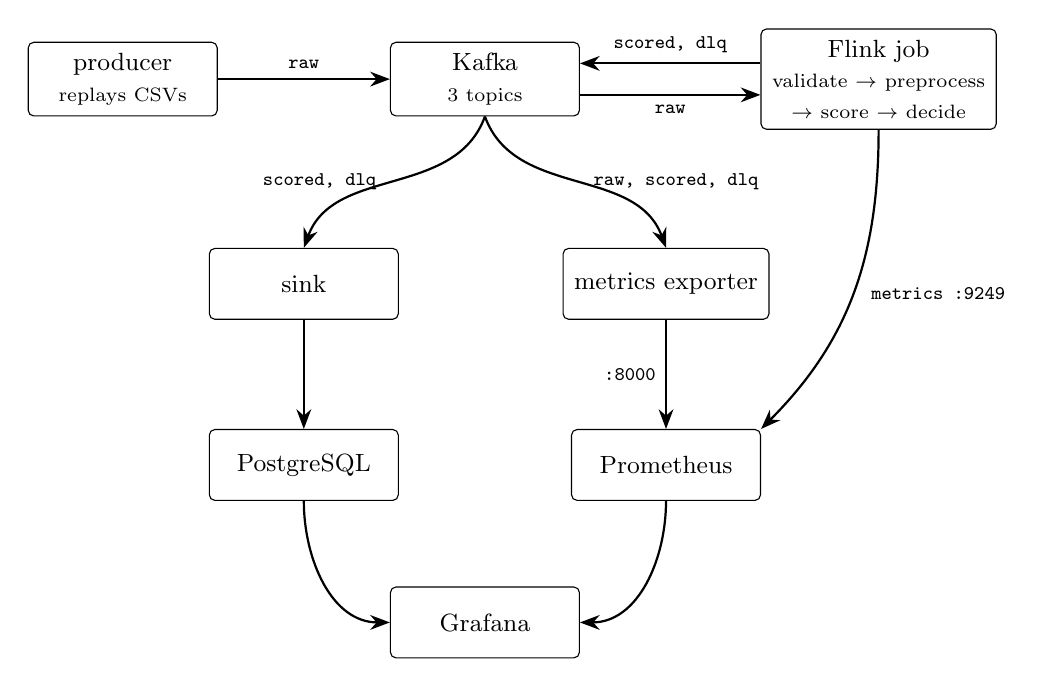
\begin{tikzpicture}[
  svc/.style={draw, rounded corners=2pt, align=center, minimum height=9mm,
              minimum width=24mm, inner sep=4pt, font=\small},
  topic/.style={font=\scriptsize\ttfamily, midway},
  arr/.style={-{Stealth[length=2.5mm]}, thick}
]
\node[svc] (producer) at (0,0)    {producer\\\scriptsize replays CSVs};
\node[svc] (kafka)    at (4.6,0)  {Kafka\\\scriptsize 3 topics};
\node[svc] (flink)    at (9.6,0)  {Flink job\\\scriptsize validate $\to$ preprocess\\\scriptsize $\to$ score $\to$ decide};
\node[svc] (sink)     at (2.3,-2.6) {sink};
\node[svc] (exporter) at (6.9,-2.6) {metrics exporter};
\node[svc] (pg)       at (2.3,-4.9) {PostgreSQL};
\node[svc] (prom)     at (6.9,-4.9) {Prometheus};
\node[svc] (graf)     at (4.6,-6.9) {Grafana};

\draw[arr] (producer) -- node[topic, above] {raw} (kafka);
\draw[arr] ([yshift=-2mm]kafka.east) -- node[topic, below] {raw} ([yshift=-2mm]flink.west);
\draw[arr] ([yshift=2mm]flink.west)  -- node[topic, above] {scored, dlq} ([yshift=2mm]kafka.east);
\draw[arr] (kafka.south) to[out=-110,in=70]  node[topic, left,  xshift=-1mm] {scored, dlq} (sink.north);
\draw[arr] (kafka.south) to[out=-70, in=110] node[topic, right, xshift=1mm] {raw, scored, dlq} (exporter.north);
\draw[arr] (sink)     -- (pg);
\draw[arr] (exporter) -- node[topic, left] {:8000} (prom);
\draw[arr] (flink.south) to[out=-90,in=45] node[topic, right, xshift=1mm] {metrics :9249} (prom.north east);
\draw[arr] (prom.south) to[out=-90,in=0]   (graf.east);
\draw[arr] (pg.south)   to[out=-90,in=180] (graf.west);
\end{tikzpicture}
\caption{Data flow. Solid arrows are Kafka topics (\code{transactions.raw},
\code{transactions.scored}, \code{transactions.dlq}), metric scrapes, or
database writes.}
\end{figure}

\section{Pipeline components}

\subsection{Replay producer (\code{producer/})}

\code{replay\_producer.py} reads \code{test\_transaction.csv} in chunks of
20{,}000 rows, attaches the matching \code{test\_identity.csv} record by
\code{TransactionID}, renames hyphenated identity columns (\code{id-01}
$\to$ \code{id\_01}), converts missing values to JSON \code{null}, and sends
one JSON object per message to \code{transactions.raw} at a configurable rate
(50 events/s by default), looping over the file when it ends. No labels are
sent, as in production. To exercise the dead-letter path, a configurable
fraction of messages (200 per million by default) is truncated into invalid
JSON. The Kafka producer batches messages (\code{linger.ms} 20,
\code{batch.num.messages} 1000) with lz4 compression.

\subsection{Kafka broker (\code{kafka}, \code{topics-init})}

A single Apache Kafka 3.9.0 broker runs in KRaft mode, acting as both broker
and controller. Automatic topic creation is disabled; a one-shot
\code{topics-init} container creates the three topics, each with one partition
and replication factor~1, and exits. Services inside the Compose network reach
the broker at \code{kafka:9092}; tools on the host use the external listener
\code{localhost:29092}.

\subsection{Flink job (\code{serving/})}

\code{flink\_job.py} defines the job \code{fraud-detection-scoring}, submitted
once by the \code{job-submit} container to a JobManager/TaskManager pair built
from \code{serving/Dockerfile} (Flink 2.1.0 on Java 17 with Python 3.12 and
PyFlink). Each event passes through four stages:

\begin{enumerate}
  \item \textbf{Validate} (\code{ValidateFunction}, logic in
  \code{schemas.py}): parse the JSON, require a non-empty object with a usable
  \code{TransactionID}, trim whitespace from keys and normalize \code{id-XX}
  keys. Failures go to a side output that is written to
  \code{transactions.dlq} with the error reason and the original payload ---
  bad input never stops the job.
  \item \textbf{Preprocess} (\code{ScoreFunction} in \code{scoring\_udf.py}):
  build the complete raw row required by the data contract (missing columns as
  null, numerics coerced to float, categoricals to strings), apply the fitted
  scikit-learn pipeline, and select the 30 model features.
  \item \textbf{Score}: the three base models each produce a fraud
  probability; the meta-learner combines them (in the order XGBoost, LightGBM,
  CatBoost) into the final probability. The models are loaded from
  \code{artifacts/} once per operator instance, in \code{open()}.
  \item \textbf{Decide and publish}: probability $\geq 0.2883 \Rightarrow$
  \code{ALERT}, otherwise \code{PASS}; any scoring error $\Rightarrow$
  \code{REVIEW} with the error message. The result is written to
  \code{transactions.scored}.
\end{enumerate}

The job checkpoints every 30 seconds in exactly-once mode and runs with
parallelism 1 on a TaskManager with 2 task slots. Both Flink processes expose
metrics to Prometheus on port 9249.

\subsection{PostgreSQL sink (\code{sink/})}

\code{consumer\_sink.py} consumes \code{transactions.scored} and
\code{transactions.dlq} (consumer group \code{scored-sink}) and writes them to
the \code{scored\_transactions} and \code{dlq\_events} tables, created from
\code{schema.sql} when the PostgreSQL container first starts. Rows are
collected into batches (500 rows or 2 seconds) and inserted in one database
transaction. Data persists across restarts in the \code{pgdata} Docker volume.

\subsection{Metrics exporter (\code{monitoring/exporter/})}

\code{metrics\_exporter.py} consumes all three topics (consumer group
\code{metrics-exporter}) and serves Prometheus metrics on port 8000:
throughput counters, score and latency histograms, the fraud flag rate, the
fallback (\code{REVIEW}) rate, the consumer lag of the scoring job, and drift.
Drift is measured in \code{drift.py} as the Population Stability Index (PSI)
over a 5-minute rolling window, for the score distribution and for ten input
features, against a reference built either from the training data
(\code{tools/make\_reference.py}) or, when no reference file exists, from the
first live events.

\subsection{Prometheus and Grafana (\code{monitoring/})}

Prometheus scrapes four targets every 15 seconds --- the Flink JobManager and
TaskManager, the metrics exporter, and itself --- and evaluates the six alert
rules in \code{alert\_rules.yml} (scoring latency, dead-letter spike, exporter
down, flag rate out of bounds, score PSI breach, fallback-rate spike). Grafana
provisions two data sources (Prometheus and PostgreSQL) and one dashboard,
\textbf{Fraud Detection}, with two rows: \emph{Transactions} (counters, a live
feed of scored transactions and the latest fraud alerts, from PostgreSQL) and
\emph{Model behavior} (decisions per second, flag rate, score PSI, fallback
rate, from Prometheus).

\section{Component interaction}

\subsection{Kafka topics}

Kafka decouples the components: no service calls another directly; everything
flows through the three topics.

\begin{table}[h]
\centering
\small
\begin{tabular}{@{}lll@{}}
\toprule
Topic & Written by & Read by (consumer group) \\
\midrule
\code{transactions.raw}    & producer  & Flink job (\code{fraud-scoring}), exporter (\code{metrics-exporter}) \\
\code{transactions.scored} & Flink job & sink (\code{scored-sink}), exporter (\code{metrics-exporter}) \\
\code{transactions.dlq}    & Flink job & sink (\code{scored-sink}), exporter (\code{metrics-exporter}) \\
\bottomrule
\end{tabular}
\caption{Topics and their producers and consumers.}
\end{table}

Because the sink and the exporter use different consumer groups, each receives
every message independently; the exporter can restart without affecting
persistence, and vice versa.

\subsection{Delivery guarantees}

\begin{itemize}
  \item \textbf{Flink}: checkpoints every 30 s in exactly-once mode for its
  internal state; the Kafka \emph{outputs} are at-least-once, so after a
  recovery some results can be published again. The source starts from the
  earliest offset, so a newly submitted job re-reads the retained events.
  \item \textbf{Sink}: Kafka offsets are committed only after the database
  transaction commits, so rows are durable before their offsets advance.
  Scored rows are inserted with \code{ON CONFLICT (transaction\_id,
  processing\_ts) DO NOTHING}, so a message redelivered after a crash is not
  stored twice. An event re-scored by Flink has a new \code{processing\_ts}
  and is stored as a separate, traceable row.
  \item \textbf{Fail-open paths}: malformed input goes to
  \code{transactions.dlq} instead of crashing the job, and inference errors
  yield \code{REVIEW} decisions instead of dropped events. Both paths are
  persisted, displayed on the dashboard, and covered by alert rules.
\end{itemize}

\subsection{Startup order}

Docker Compose starts the services in dependency order: \code{kafka} and
\code{postgres} first (both health-checked); then \code{topics-init} creates
the topics and exits; \code{jobmanager} starts once Kafka is healthy;
\code{taskmanager} and \code{job-submit} wait for a healthy JobManager (and
\code{job-submit} for the topics); \code{producer}, \code{sink} and
\code{metrics-exporter} wait for the topics (the sink also for a healthy
PostgreSQL); \code{prometheus} starts after the exporter and \code{grafana}
after Prometheus.

\section{Dashboard walkthrough}

The Grafana dashboard has two rows. The screenshots below come from a live
run of the stack, replaying at a few events per second.

\subsection{Transactions row}

\begin{figure}[h]
\centering
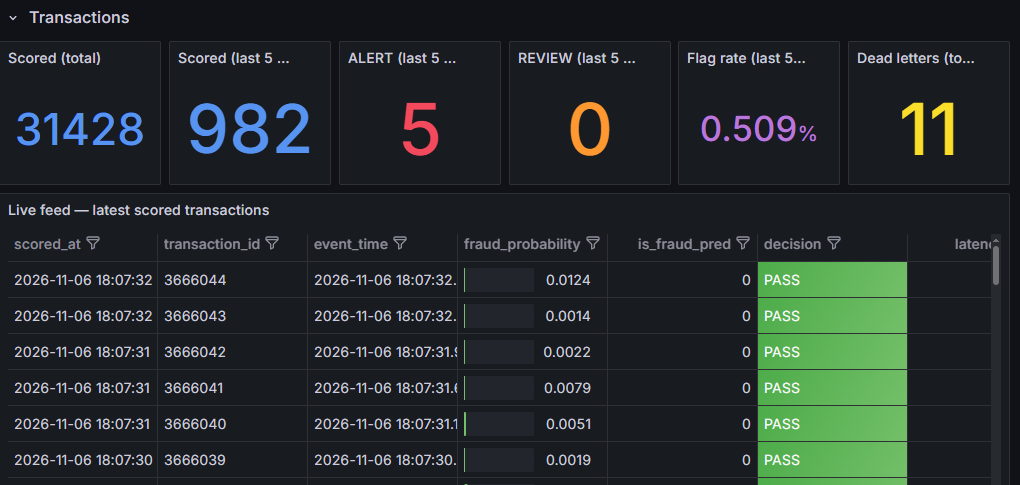
\includegraphics[width=\textwidth]{dashboard-transactions.png}
\caption{Transactions row during a live run: the six counters and the top of
the live feed.}
\label{fig:transactions}
\end{figure}

This row is built from SQL queries against PostgreSQL, so it shows what has
actually been persisted, not just what passed through Kafka. The six stat
panels have no axes; each shows a single current value:

\begin{itemize}
  \item \textbf{Scored (total)} --- all rows in \code{scored\_transactions}
  since the database volume was created (31{,}428 in the screenshot; the
  producer loops over the replay file, so this grows without bound).
  \item \textbf{Scored (last 5 min)} --- rows inserted in the last five
  minutes (982 here, about 3.3 events per second).
  \item \textbf{ALERT (last 5 min)} and \textbf{REVIEW (last 5 min)} ---
  decisions of each type in the same window (5 alerts, 0 reviews).
  \item \textbf{Flag rate (last 5 min)} --- the mean of \code{is\_fraud\_pred}
  over the window (0.509\%, which is $5/982$; at this low event rate a single
  alert moves the rate visibly, which is why the alert rule tolerates
  0.5--15\%).
  \item \textbf{Dead letters (total)} --- all rows in \code{dlq\_events}
  (11 here, consistent with the producer's default injection of about 200
  malformed events per million).
\end{itemize}

Below the counters, the \emph{live feed} table lists the most recently scored
transactions, newest first: \code{scored\_at} and \code{event\_time} (the
scoring time, derived from \code{processing\_ts}), the \code{transaction\_id},
the \code{fraud\_probability} drawn as a small gauge (green until it
approaches the 0.2883 threshold, red beyond it), the binary
\code{is\_fraud\_pred}, the color-coded \code{decision} (green \code{PASS},
red \code{ALERT}, orange \code{REVIEW}), and the scoring latency. In the
screenshot all visible rows are low-probability \code{PASS} decisions, which
is the expected steady state at a fraud rate of about 3.5\%.

\subsection{Model behavior row}

\begin{figure}[h]
\centering
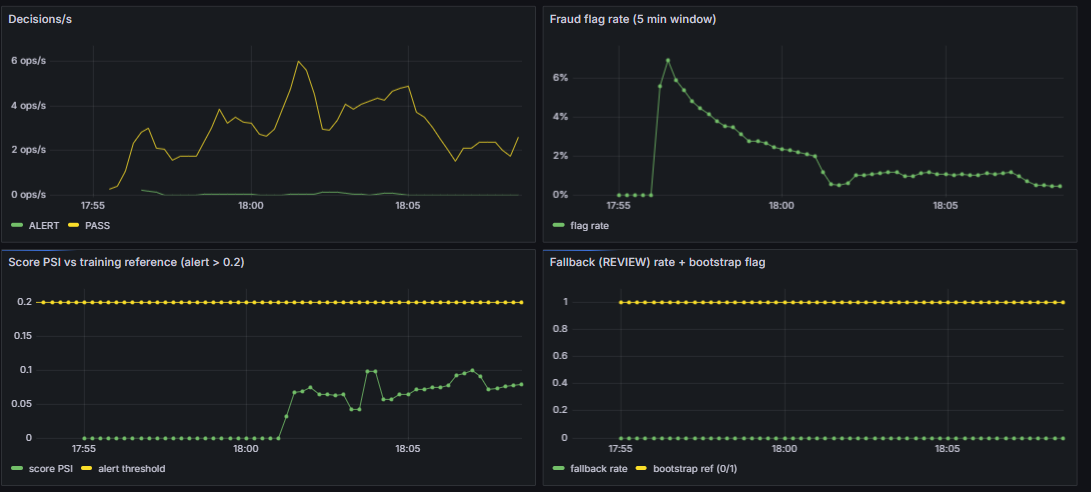
\includegraphics[width=\textwidth]{dashboard-model-behavior.png}
\caption{Model behavior row during the same run.}
\label{fig:modelbehavior}
\end{figure}

All four panels are time series from Prometheus; the x-axis is wall-clock
time in every panel.

\begin{itemize}
  \item \textbf{Decisions/s} --- y-axis: scored events per second, one line
  per decision. This is the scoring throughput split by outcome; \code{ALERT}
  should run far below \code{PASS}. In the screenshot, 2--6 events per second
  of \code{PASS} with \code{ALERT} near zero.
  \item \textbf{Fraud flag rate (5 min window)} --- y-axis: the share of
  flagged transactions in a rolling five-minute window, in percent. A sanity
  check on the model: a rate collapsing to zero or exploding signals a broken
  model or feed even while throughput looks normal. The early spike to about
  7\% in the screenshot is small-sample noise while the window is still
  filling; it settles near 1\%, inside the 0.5--15\% alert bounds.
  \item \textbf{Score PSI vs training reference} --- y-axis: the Population
  Stability Index of the score distribution (unitless); the horizontal line
  marks the 0.2 alert threshold. Values below 0.1 are read as stable, 0.1--0.2
  as a moderate shift, above 0.2 as a significant shift. The screenshot shows
  PSI between 0.05 and 0.10 --- stable.
  \item \textbf{Fallback (REVIEW) rate + bootstrap flag} --- y-axis:
  dimensionless 0--1. The fallback rate is the share of \code{REVIEW}
  decisions in the window (flat at zero here: no inference errors). The
  second series is a 0/1 status flag, not a rate: 1 means no
  \code{reference\_distributions.json} was found, so the drift reference was
  bootstrapped from the first live events of this run rather than from the
  training data. This also explains why the PSI starts at exactly zero: the
  earliest window is compared against itself.
\end{itemize}

\subsection{Fail-open design: \code{REVIEW} and dead letters}

The pipeline is designed never to drop a transaction, and \code{REVIEW} and
the dead-letter queue are the two halves of that guarantee, covering two
different failure modes.

\textbf{Dead letters} handle bad \emph{input}. A message that is not valid
JSON, not an object, or has no usable \code{TransactionID} cannot be scored at
all. Without a dead-letter path, such a message either crashes the Flink job
--- which then restarts onto the same message in an endless loop, halting all
scoring --- or is silently discarded. Instead, the validation stage routes it
to \code{transactions.dlq} with the error reason and the original payload; it
is persisted in the \code{dlq\_events} table, counted on the dashboard, and
covered by the \code{DlqSpike} alert. The producer deliberately injects
malformed messages (about 200 per million) so this path is always exercised.

\textbf{\code{REVIEW}} handles \emph{inference} failure. The input parsed
correctly, but something went wrong while scoring --- an unconvertible value,
a library error, a corrupt artifact. Dropping the event would let a payment
through with no decision at all, so the event is published anyway, with a
null probability, the error message, and the decision \code{REVIEW}: a real
transaction handed to a human because the model could not score it. The
\code{FallbackRateSpike} alert fires if more than 1\% of traffic takes this
path, which would indicate a broken model deployment.

The two are easy to distinguish: a dead letter was never a readable
transaction; a \code{REVIEW} is a readable transaction that received no
score. Both are persisted, visible on the dashboard, and alerted on.

\clearpage

\section{Project layout}

\begin{table}[h]
\centering
\small
\begin{tabular}{@{}p{0.34\textwidth}p{0.58\textwidth}@{}}
\toprule
Path & Purpose \\
\midrule
\code{.github/workflows/tests.yml} & Continuous integration: runs the 30-test
  \code{pytest} suite on every push and pull request. \\
\code{artifacts/} & The trained model bundle the serving code depends on:
  three base models in native formats, the XGBoost meta-learner, the pickled
  preprocessing pipeline, the selected features, the decision threshold, and a
  manifest recording versions, data hashes, hyperparameters and held-out
  metrics. \\
\code{assets/} & Dashboard screenshots referenced by the README. \\
\code{data/} & The replay CSVs downloaded from Kaggle
  (\code{test\_transaction.csv}, \code{test\_identity.csv}); not tracked by
  git. \\
\code{docs/} & Project documentation: \code{PROJECT.md} (full technical
  documentation), \code{operations.md} (operating guide), and this document. \\
\code{monitoring/} & Everything observability: \code{exporter/} (the
  model-behavior metrics exporter and PSI drift code), \code{grafana/}
  (the provisioned dashboard and the data-source/dashboard provisioning
  files), \code{alert\_rules.yml} (six Prometheus alert rules) and
  \code{prometheus.yml} (scrape configuration). \\
\code{notebook/} & The two Kaggle notebooks: exploratory data analysis and
  model training. Training exports the \code{artifacts/} bundle and reports
  the held-out metrics. \\
\code{producer/} & The replay producer and its Dockerfile. \\
\code{serving/} & The Flink job: job wiring (\code{flink\_job.py}), event
  validation (\code{schemas.py}), the scoring operator
  (\code{scoring\_udf.py}) and the Dockerfile that builds the Flink image with
  Python, PyFlink, the ML libraries and the Kafka connector. \\
\code{sink/} & The Kafka-to-PostgreSQL consumer and the database schema. \\
\code{tests/} & 30 \code{pytest} tests across five modules: schema validation,
  scoring, training/serving preprocessing parity, the metrics exporter, and
  the sink. \\
\code{tools/make\_reference.py} & Builds the drift reference distributions
  from the training data. \\
\code{docker-compose.yml} & Defines the eleven services of the full stack. \\
\code{docker-compose.lowmem.yml} & Overrides for hosts with 8\,GB RAM. \\
\code{requirements-serve.txt} & Pinned serving and test dependencies. \\
\bottomrule
\end{tabular}
\caption{Repository layout.}
\end{table}

\clearpage

\appendix

\section{The technologies}

\subsection{Apache Kafka}

Kafka is a distributed event log. Producers append messages to named
\emph{topics}; consumers read them at their own pace, tracked by an
\emph{offset} per \emph{consumer group}, so several independent readers can
each receive every message. Messages are retained on disk for a configured
time regardless of whether they have been read, which allows replay and
late-joining consumers. Topics are split into \emph{partitions} for
parallelism and replicated across brokers for durability. In this project a
single broker in KRaft mode (Kafka's built-in consensus, replacing ZooKeeper)
carries three single-partition topics; Kafka's role is to decouple the
producer, the scoring job, the persistence sink and the metrics exporter, so
each can fail, restart or lag independently.

\subsection{Apache Flink}

Flink is a distributed stream processor: it runs continuous jobs over
unbounded streams, processing events one at a time with millisecond-level
latency (in contrast to micro-batch engines such as Spark Structured
Streaming). A \emph{JobManager} coordinates the job and a \emph{TaskManager}
executes its operators in task slots. Flink's defining feature is managed
state with periodic \emph{checkpoints}: a consistent snapshot of all operator
state and source offsets, from which the job restarts automatically after a
failure --- exactly-once semantics for the internal state. PyFlink is the
Python API used here; the job consumes from Kafka, applies a validation
operator and a Python scoring operator holding the loaded ML models, and
produces to Kafka. This project chose Flink because fraud scoring is
per-event and latency-sensitive.

\subsection{Docker and Docker Compose}

Docker packages an application with its exact dependencies into an
\emph{image}, which runs as an isolated \emph{container} sharing the host's
kernel. This pins the entire runtime --- OS libraries, Python version, ML
library versions --- so the stack behaves identically on any machine. Docker
Compose describes a multi-container application in one YAML file: the
services, the images to build or pull, environment variables, mounted
volumes, published ports, health checks and start-up dependencies. Here,
\code{docker-compose.yml} defines the eleven services, their start order and
a named volume for the database, so \code{docker compose up --build -d}
brings up the entire pipeline; \code{docker-compose.lowmem.yml} overlays
smaller memory limits for 8\,GB hosts.

\subsection{Prometheus}

Prometheus is a time-series database built for monitoring. It works by
\emph{pulling}: every scrape interval (15\,s here) it fetches the current
values from each target's \code{/metrics} HTTP endpoint and stores them with
timestamps. Metrics come in a few types --- counters, gauges and histograms
--- and are queried with PromQL, which computes rates, quantiles and
aggregations over time (for example, the p99 scoring latency over the last
five minutes from a histogram). Prometheus also evaluates \emph{alerting
rules}: expressions that, when true for a configured duration, raise an
alert. In this project it scrapes the Flink processes and the metrics
exporter and evaluates the six alert rules; active alerts are visible in its
web UI.

\subsection{Grafana}

Grafana is a visualization layer: it queries data sources --- here Prometheus
and PostgreSQL --- and renders the results as dashboards of panels (time
series, stats, tables) that refresh continuously. Dashboards and data
sources can be \emph{provisioned} from files on disk, which is how this
project ships its dashboard: the JSON definition and the data-source
configuration live in the repository and are mounted into the container, so
a fresh \code{docker compose up} yields a fully configured dashboard with no
manual clicks. The single dashboard combines SQL queries against the scored
transactions (live feed, counters) with PromQL queries (rates, PSI) in one
view.

\end{document}
